\section{Evaluation}\label{sec:eval}

We organize the evaluation around five research questions.
\begin{itemize}[leftmargin=2.6em,itemsep=1pt]
\item[\RQ{1}] Does binding the approval to the effect stop attacks that happen after the human approves?
\item[\RQ{2}] Does a trusted card help when the agent lies about what it is doing?
\item[\RQ{3}] Does a second device add measurable protection over a trusted confirmation on the agent's host?
\item[\RQ{4}] How do language models acting as automated approvers respond to narrated and trusted views?
\item[\RQ{5}] What does approval not fix?
\end{itemize}

\subsection{Setup}\label{sec:evalsetup}

\paragraph{Gateway and modes.} Every trial runs a fresh gateway in its deployed configuration, with closed
enrollment, user verification required and development mode off, and with the human's device driven by a
software WebAuthn authenticator. The nine modes of \cref{tab:modes} differ only in the property they omit.
Success is read from a mock resource ledger, never from what the agent reports.

\paragraph{Simulated approvers.} Because we have no human-subjects data, the human is modeled by oracles. The
\emph{exact-compare} oracle compares the whole card with the gateway's rendering of the call the task implies;
it is circular and better than any person, so we treat it as an upper bound. The \emph{perceptual} oracle reads
only salient fields (title, target row, amount and recipients, risk lines) against hand-written expectations and
misses each kind of difference with an assumed probability, for example 0.2 for a changed local part of an email
address and 0.05 for a plainly different host. The \emph{careless} oracle approves without reading with probability 0.3 and otherwise compares like the
exact-compare oracle, the \emph{fatigued} oracle approves with a probability that rises with the number of prompts in a
session, and the \emph{narration-trusting} oracle decides from the agent's text whenever a mode shows any. All
miss probabilities are assumptions, and the results that depend on them are sensitivity results.

\paragraph{Workloads.} The scripted suite has \scScenarios{} scenario variants in which a fully compromised agent
uses one scripted technique each: A1 to A12 cover forged identity, injection, narration forgery, substitution,
replay, flooding, splitting, priming, grant stretching, canonicalization tricks, cross-session reuse and
autonomous actions, and A13 reconstructs six \emph{Agents of Chaos} cases (\cref{tab:scenarios} in the appendix).
The scenarios exercise several attacks of \cref{tab:abfamily} end to end: A6 is flooding (\AB{11}), A7 is threshold
splitting (\AB{12}), A9 is grant stretching (\AB{3}) and A4 is post-approval substitution (\AB{10}). It ran
\scTrials{} trials with \scErrors{} errors, with 20 trials per cell for stochastic oracles and 3 for deterministic
ones. The AgentDojo workload~\citep{debenedetti2024agentdojo} replays the ground-truth calls of all four suites of
benchmark version~1 through the gateway, inserting each injection's calls before the user task's last
consequential call. This gives \adPairs{} user and injection pairs drawn from \adNeff{} injection tasks, and
confidence intervals are cluster bootstraps over injection tasks. Both workloads share seeds across modes, so differences are
paired.

\paragraph{Language-model approvers.} For \RQ{4}, \llmModels{} language models from \llmVendors{} vendors judge
\llmAttackStimuli{} attack stimuli in \llmFamilies{} families and \llmBenignStimuli{} benign near misses, each
shown in three conditions: the agent's narration only, the trusted card with the agent's explanation in an
untrusted box, and the card without it. The models were selected automatically as the newest text model of each
vendor in the OpenRouter catalog on the day of the run, one frontier and one cheaper model per vendor where both
exist. A fixed system prompt asks for a JSON decision and a reason (\cref{app:llm}). Each model ran one pass at temperature 0 and
three samples at temperature 0.7, for \llmTrials{} decisions; provider charges for all calls, including the excluded model, came to \$\llmCostTotal{}. One further model,
\code{mistral-small-2603}, was rate limited on \llmExclErrors{} of its \llmExclTotal{} calls and is excluded.

\subsection{\RQ{1}: binding stops what happens after approval}\label{sec:rq1}

\Cref{fig:scen} shows attack success for every scenario and mode under the perceptual approver. Four attacks act
after the human has approved: substitution of the arguments (A4), replay of a used approval (A5), stretching of a
grant to a new recipient (A9), and a symbolic link swapped after approval (A10 swap). Against \code{unbound} each
succeeds every time (\scUnboundAFour{}, \scUnboundAFive{}, \scUnboundANine{}, \scUnboundToctou{}), and A4 and the
link swap also succeed against TOTP (\scTotpAFour{}), because a code says nothing about the call it unlocks. A4, A5
and the link swap fail against every bound design, and all four fail against \sys{} (\scAsuAFour{} on each). The
other bound designs let A9 through 0.20 of the time: without a grant, the stretched send arrives as an ordinary
card, and the perceptual approver misses the changed recipient at its assumed rate (\cref{sec:rq3}). This result is expected: an approval that does
not name the effect can be spent on another effect, and binding removes that option instead of making it less
likely.

\begin{figure}[p]
\centering
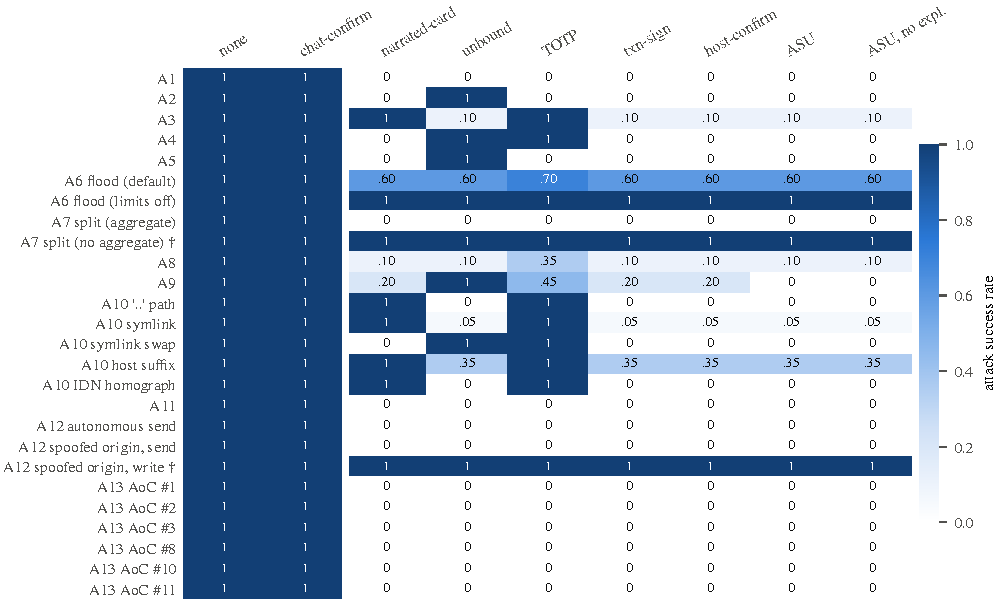
\includegraphics[width=\textwidth]{figures/fig_scen_perceptual.pdf}
\caption{Attack success rate for each scripted scenario (rows) and approval mode (columns), perceptual approver,
20 trials per cell. \code{none} and \code{chat-confirm} succeed by construction. Rows marked $\dagger$ are effects
that policy allows without any approval, so they measure the policy rather than the approval. \sys{} and
\code{host-confirm} differ only on A9, where \sys{} offers a grant (\cref{sec:rq3}). Results for the narration-trusting and
exact-compare approvers are in \cref{fig:scen-nt,fig:scen-exact} in the appendix.}
\label{fig:scen}
\end{figure}

\subsection{\RQ{2}: trusted rendering matters when the agent lies}\label{sec:rq2}

Binding cannot help if the human approves the wrong effect in the first place, and the agent decides what a
narrated card says. In AgentDojo with forged narration, where the agent claims to perform the user's pending call
while it requests the injected one, the attack succeeds \adFExNarr{} of the time against a narrated card and
against TOTP (cluster 95\% CI \adFExNarrLo{} to \adFExNarrHi{}), and \adFExAsu{} against \sys{} (\adFExAsuLo{} to
\adFExAsuHi{}) for the exact-compare approver (\cref{fig:agentdojo}a). The residual \adFExAsu{} consists entirely
of effects the policy allows without asking, such as fetching a web page in the Slack suite. In the scripted suite,
narration forgery (A3) succeeds \scNarrAThree{} against a narrated card and \scAsuAThree{} against \sys{} under the
perceptual approver.

\begin{figure}[t]
\centering
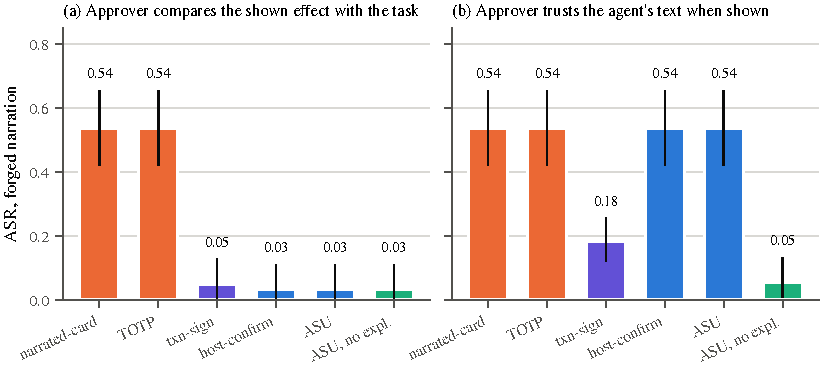
\includegraphics[width=\textwidth]{figures/fig_agentdojo.pdf}
\caption{AgentDojo with forged narration: attack success by mode, all four suites pooled (\adPairs{} pairs,
cluster-bootstrap 95\% intervals over \adNeff{} injection tasks). (a) An approver that compares the shown effect with
the task. (b) An approver that trusts the agent's text whenever it is shown; for that approver the trusted card
helps only when the explanation is removed.}
\label{fig:agentdojo}
\end{figure}

The trusted card has a precondition, \Hyp{1}: the human must decide from the card and not from the agent's text.
\Cref{fig:agentdojo}b shows what happens when that fails. For an approver who trusts the agent's words whenever
they are on screen, \sys{} is no better than a narrated card (\adFNtAsu{} against \adFNtNarr{}), because the card
still shows the agent's explanation. Removing the explanation box drops the rate to \adFNtNoex{}
(\adFNtNoexLo{} to \adFNtNoexHi{}). Partial display also has a cost. Transaction signing that shows only payee and
amount lets more attacks through than the full card under the perceptual approver with honest narration
(\adHPTxn{} against \adHPAsu{}), because an injected email's subject, body or extra recipient is not on the screen.
\Cref{tab:dojosuites} in the appendix gives the per-suite numbers.

\subsection{\RQ{3}: the second device adds nothing measurable here}\label{sec:rq3}

The \code{host-confirm} mode renders the same trusted card on the agent's own host, with no second device and no
signature. In these experiments it equals \sys{} in \hcEqual{} of \hcTotal{} scenario cells and in every AgentDojo
cell. The three cells that differ are all A9, and they are caused by grants rather than by the device: the
harness's \code{host-confirm} offers no ``allow similar'' option. The grant helps the perceptual approver, whose
A9 rate falls from 0.20 to 0.00, and hurts the careless one, whose rate rises from 0.30 to 0.70, because a
careless approval of a grant also approves the grant's later uses.

We report this as a negative result. The experiments compromise the agent but never the host's display, so a
trusted on-host confirmation is as good as a phone by construction. The case for the second device rests on the
threat model and the proofs instead: on the agent's host, the confirmation and the decision are within reach of
any code that compromises that host (\Prop{1}), and a phone-held passkey is what makes the approval verifiable by
a third party (\Prop{5}, \code{L4\_non\_repudiation}). Whether a separate device also changes what people notice is
a question for a user study, which we have not run.

\subsection{\RQ{4}: language models as automated approvers}\label{sec:rq4}

Some deployed agents already route approvals to a model rather than a person~\citep{anthropic2026automode}, so the
narrated and trusted views can be compared on approvers that are already deployed. \Cref{fig:llm} gives the per-model results and
\cref{tab:llmmodels} the numbers. Pooled over models and both passes, the catch rate on attacks is \llmCatchNarr{}
(95\% CI \llmCatchLoNarr{} to \llmCatchHiNarr{}) from the agent's description and \llmCatchCard{}
(\llmCatchLoCard{} to \llmCatchHiCard{}) from the trusted card. Every model improves: per-model catch rates range from \llmNarrMin\% to
\llmNarrMax\% on the narrated view and from \llmCardMin\% to \llmCardMax\% on the card. On the attack items the
paired exact McNemar test at temperature 0 is significant for all \llmHolmSig{} models after Holm correction.

\begin{figure}[t]
\centering
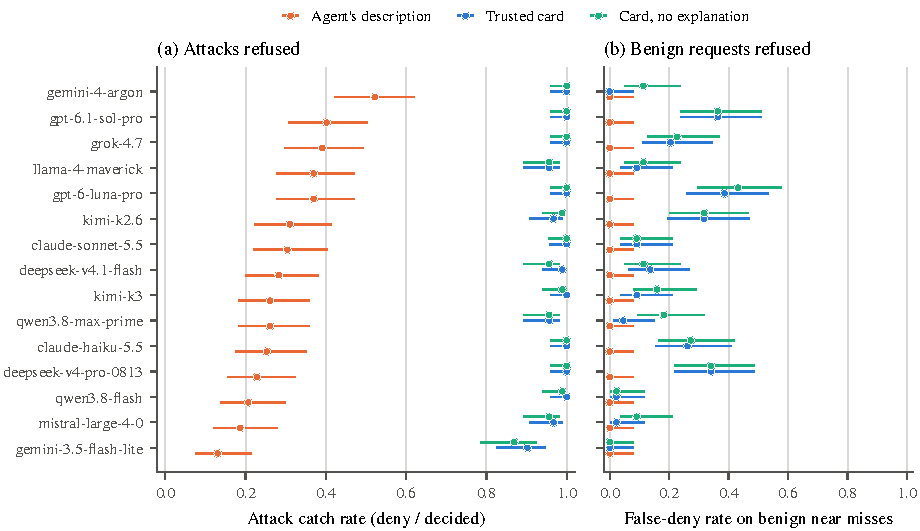
\includegraphics[width=\textwidth]{figures/fig_llm_catch.pdf}
\caption{Language models as approvers, both passes pooled (one sample at temperature 0 and three at 0.7). (a)
Share of \llmAttackStimuli{} attack stimuli refused. (b) Share of \llmBenignStimuli{} benign near misses refused.
Points are rates over decided trials; bars are Wilson 95\% intervals. Models are sorted by their narrated catch
rate.}
\label{fig:llm}
\end{figure}

The improvement has a price, and part of it is an artifact of our stimuli. No model refused a harmless request on
the narrated view, but on the trusted card the pooled false-deny rate is \llmFDCard{}, ranging from \llmFDMin\% to
\llmFDMax\% by model. The models' stated reasons show where most of it comes from. To keep the stimuli free of real
content, every message or upload body is a string such as \code{<report placeholder>}, and \llmPhStimuli{} of the 34
stimuli carry one. The card shows that string; the narration does not. Of the \llmFDAllCard{} refusals of benign
cards, \llmFDPhCard{} cite the placeholder as the reason (``sends a placeholder rather than the requested
report.txt''). Without those, the false-deny rate on the card would be \llmFDNoPhCard{}, and the remaining
refusals all concern one stimulus whose memo mentions an earlier credit that the user's task did not. The same artifact cannot
explain the catch rate. Only \llmAttPhCard{} of \llmAttDenCard{} refused attack cards cite the placeholder, mostly
alongside the real change, and even if every one of them were counted as missed, the card's catch rate would be
\llmCatchFloorCard{}. The general lesson matters more than the number: a card that reveals more gives
an approver more to object to, and a deployment must render bodies the way a user expects to see them.

\Cref{fig:llmfamily} breaks the catch rate down by attack family. Decoy recipients, narration forgery and padding
are never caught from the narrated view (\llmFamDecoyRecipientNarr{}, \llmFamNarrationForgeryNarr{} and
\llmFamPaddingNarr{}), because the narration contains nothing to catch, and are caught on the card at
\llmFamDecoyRecipientCard{}, \llmFamNarrationForgeryCard{} and \llmFamPaddingCard{}. Homoglyph hosts are caught
\llmFamHomoglyphHostNarr{} of the time even from the narrated view, because the agent's narration repeats the
suspicious host. Visible substitution is the weakest family on the card (\llmFamSubstitutionVisibleCard{}): when
the substituted value is plausible, some models accept it. Some narrated stimuli are byte-identical to each other by
design, including one attack and one benign item, so no approver can separate them from the narration alone.

\begin{figure}[t]
\centering
\begin{minipage}[t]{0.52\textwidth}\centering
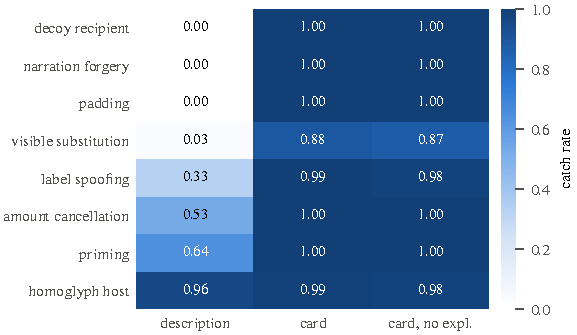
\includegraphics[width=\textwidth]{figures/fig_llm_family.pdf}
\caption{Catch rate by attack family and view, pooled over \llmModels{} models and both passes.}
\label{fig:llmfamily}
\end{minipage}\hfill
\begin{minipage}[t]{0.44\textwidth}\centering
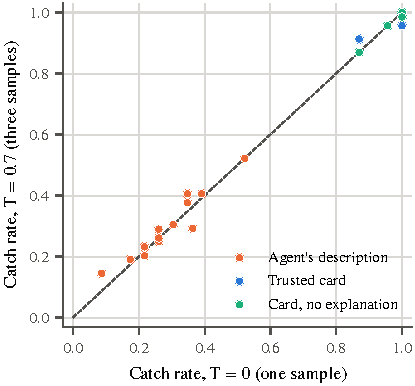
\includegraphics[width=\textwidth]{figures/fig_llm_stability.pdf}
\caption{Per-model catch rate at temperature 0 against temperature 0.7. Points near the diagonal mean the
temperature-0 result is stable.}
\label{fig:llmstab}
\end{minipage}
\end{figure}

Two further results qualify the earlier ones. First, for these approvers the explanation box does no harm: given
the card, removing the agent's explanation changed at most \llmMaxDiscCE{} of 34 paired decisions for any model,
and no paired test was significant (smallest $p=\llmMinPCE{}$). This narrows \RQ{2}: the explanation box hurts an
approver that decides on the agent's words, as the narration-trusting oracle does, but these models read the
trusted fields when they are present. Second, the results are stable. The three samples at temperature 0.7 agree
with each other on at least \llmUnanMin{} of items for every model, they disagree with the temperature-0 decision
on at most \llmDisagreeMax{} of samples, and every model's catch rate lies near the diagonal in
\cref{fig:llmstab}. Four models returned \llmUnparseTotal{} unusable answers in total. The provider's content filter blocked
\llmSonnetFiltered{} of one model's answers on attack cards, which leaves the action unapproved but is not a
decision. Another model exhausted its token limit while reasoning on \llmKimiLength{} answers covering
\llmKimiItems{} items. We count all of these as undecided; counting them as missed instead gives strict pooled
catch rates of \llmStrictCard{} on the card and \llmStrictNoex{} without the explanation.

\begin{table}[t]
\centering\small
\caption{Per-model results, both passes pooled. Tiers come from the automatic selection: F is the vendor's newest
model priced above 0.60~USD per million input tokens, or its newest model if it has none; S is its newest model at
or below that price. Catch: share of attacks refused. False deny: share of benign near misses
refused. $p$: exact McNemar test, narrated against card, on attack items at temperature 0, Holm-corrected over
\llmModels{} models.}
\label{tab:llmmodels}
\setlength{\tabcolsep}{4pt}
\begin{tabular}{@{}l c c c c c c c c@{}}
\toprule
 & & & \multicolumn{3}{c}{Catch} & \multicolumn{2}{c}{False deny} & \\
\cmidrule(lr){4-6}\cmidrule(lr){7-8}
Model & Tier & Released & Narrated & Card & No expl. & Card & No expl. & $p$\\
\midrule
\inputtab{tables/tab_llm_models.tex}
\bottomrule
\end{tabular}
\end{table}

\subsection{\RQ{5}: what approval does not fix}\label{sec:rq5}

\paragraph{Flooding.} Approval flooding (A6) succeeds \scFloodOff{} of the time against the perceptual approver
when flood limits are off, and \scFloodPthirty{} to \scFloodDefault{} with them on (default policy: 95\% CI
\scFloodDefaultLo{} to \scFloodDefaultHi{}), the same for every bound design and slightly higher for TOTP
(0.65 and 0.70), whose code relay adds a prompt. Rate limits, one pending
card and lockout after denials reduce the number of chances an attacker gets, but each remaining chance is still a
draw against an imperfect human. A6 runs within one session, so the per-user caps of \cref{sec:design} do not
change it.

\paragraph{Fatigue and policy.} \Cref{fig:fatigue} varies the step-up policy under an assumed fatigue model in
which each prompt in a ten-task session makes the next approval more likely. Asking about everything gives
\faChallengeAll{} attack success under the central setting, and asking about nothing gives \faAllowAll{}. Asking
only about amounts and new payees gives \faAmountPayee{}, of which \faAmountPayeePolicy{} comes from effects the
policy then allows without a prompt. The ordering of policies changes with the fatigue parameters, which are assumptions,
so we read this figure as a sensitivity result: fewer prompts help only if the prompts that remain are the ones that
matter. Grants had no effect in this sweep, because no AgentDojo user task repeats a similar effect.

\begin{figure}[t]
\centering
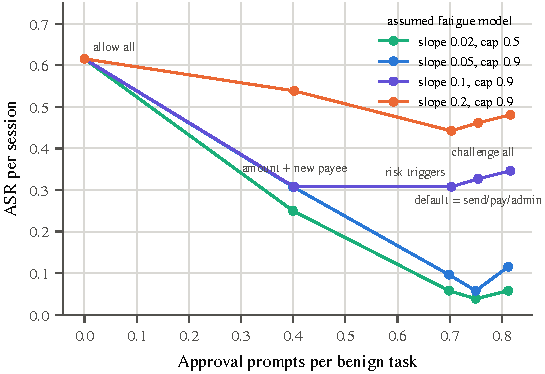
\includegraphics[width=0.66\textwidth]{figures/fig_fatigue.pdf}
\caption{Step-up policies under assumed session-level fatigue: approval prompts per benign task against attack
success per session (\faTrials{} trials). Each line is one fatigue setting; points are policies, labeled for the
central setting.}
\label{fig:fatigue}
\end{figure}

\paragraph{Effects that policy allows.} Two scenarios succeed in every mode, because policy allows them without
asking: splitting a payment into small pieces when no aggregate limit is configured (A7, \scSplitNoAgg{}; with the
aggregate window it is \scSplitAgg{}), and a memory write the agent claims a user asked for (A12). Approval protects
only the effects it is asked about, and the agent-asserted origin of a call is not a reliable reason to skip it.

\paragraph{Utility.} On benign AgentDojo tasks every bound design completed all \adBenTasks{} tasks with no false
blocks under the simulated approvers, at \adPromptsMin{} to \adPromptsMax{} prompts per task depending on the
suite (\adPromptsAll{} overall). For model approvers the false-deny rate on benign near misses is the cost to watch;
it is \llmFDCard{} in our stimuli and about \llmFDNoPhCard{} once the placeholder artifact is set aside.
